\documentclass[amsmath,amssymb,notitlepage,12pt]{revtex4}
%\documentclass[12pt]{article}
\usepackage[toc,page]{appendix}
\usepackage{graphicx}
\usepackage{bm}% bold math
\usepackage{multirow}
\usepackage{booktabs}
\usepackage{verbatim}
\usepackage{hyperref}
\usepackage{enumitem}
\hypersetup{pdftex,colorlinks=true,allcolors=blue}
\usepackage{hypcap}
\usepackage[small,compact]{titlesec}
\setlist[enumerate]{itemsep=0mm}
\addtolength{\textwidth}{1cm}
\addtolength{\hoffset}{-0.5cm}
\addtolength{\textheight}{2.0cm}
\addtolength{\voffset}{-0.0cm}
\begin{document}
\title{CLAS12 M{\o}ller Operations Manual - v0.4}
\date{\today}
\author{N. Baltzell, S. Stepanyan}
\begin{abstract}
\end{abstract}

\maketitle
%\tableofcontents
%\newpage

\section{Introduction}
The CLAS12 M{\o}ller system measures the polarization of the electron beam delivered to Hall B, and this document details its operating procedures.  The user interface for shift workers is shown in Fig.~\ref{fig:unconfig} and provides direct access to all controls and feedback that the normal operator should need, and its operating procedures are described in Section~\ref{sec:user}.  Expert operations are described in Section~\ref{sec:expert}.

\begin{figure}[htbp]\centering
    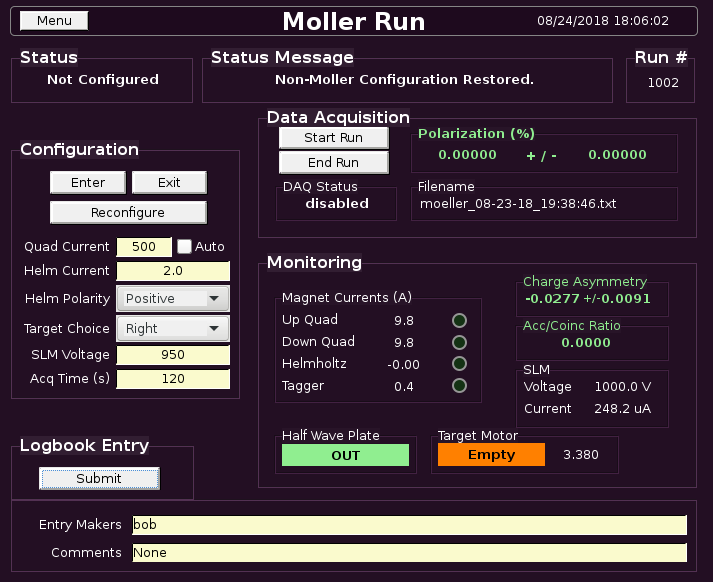
\includegraphics[width=11cm]{pics/unconfig}
    \caption{The user interface for shift workers for operating a M{\o}ller run is divided into {\em Status}, {\em Configuration}, {\em Data Acquisition}, {\em Monitoring}, and {\em Logbook} sections.  In this screenshot, the M{\o}ller system is not configured, according to the {\em Status} section, i.e. the setup is for non-M{\o}ller beam delivery.\label{fig:unconfig}}
\end{figure}

\section{Hardware Settings}
The standard hardware settings for a M{\o}ller run are shown in Table~\ref{tab:pars}.  These are displayed in the {\em Configuration} section of Figure~\ref{fig:unconfig} and will be used to automatically configure all hardware during the procedure in Section \ref{sec:user}.  It is the responsibility of the operator to ensure that the settings in the {\em Configuration} section are the desired ones before entering the M{\o}ller setup.
\begin{table}[htbp]\centering
    \begin{tabular}{ll}\toprule[1.5pt]
        SLM Voltage & 1400 V \\
        Collimator Position & Blank \\
        Target Position & Left \\
        Helmholtz Current & $\pm$3.5 A \\
        \cmidrule[0.5pt]{1-2}
        \multicolumn{2}{c}{Quadrupole Current} \\
        5-pass / 10.7 GeV & 3145 A\\
        3-pass / 6.4 GeV & 1350 A\\
        \bottomrule[1.5pt]
    \end{tabular}
    \caption{Standard hardware parameter values for the M{\o}ller setup.  Live values are shown in the {\em Monitoring} section in Figure~\ref{fig:unconfig}.\label{tab:pars}}
\end{table}

\section{Quality Requirements}\label{sec:quality}
The requirements to be maintained during a M{\o}ller run, and the resulting desired error on the polarization measurement are shown in Table~\ref{tab:reqs}.  It is the responsibility of the operator to monitor these quantities to ensure a successful polarization measurement.
\begin{table}[htbp]\centering
    \begin{tabular}{ll}\toprule[1.5pt]
        2C21 BPM Current & $\sim$4 nA\\
        Beam Charge Asymmetry & $<0.1\%$\\
        Accidental/Coincidence Ratio & $<0.05$ \\
        Final Beam Polarization Error & $<1.5\%$ (absolute)\\
        \bottomrule[1.5pt]
    \end{tabular}
    \caption{Standard quality conditions required for a M{\o}ller run.  Live values are shown in the {\em Monitoring} and {\em Data Acquisition} sections in Figure~\ref{fig:unconfig}.  Note, beam polarization error depends on statistics and should gradually decrease during the run.\label{tab:reqs}}
\end{table}

\section{Standard Procedures}\label{sec:user}

\subsection{Summary}
The procedure for the operator with the interface in Figure~\ref{fig:unconfig} can be summarized in the following steps, and more details are shown on the next section.
\begin{enumerate}
\vspace{-4mm}\item {\bf Configure:}  ensure the Configuration section is set as desired
\vspace{-4mm}\item {\bf Enter:} click {\em Enter} in the Configuration section and wait for success status
\vspace{-4mm}\item {\bf Start Run:} click {\em Start Run} in the DAQ section
\vspace{-4mm}\item {\bf Monitor:} monitor the critical parameters
\vspace{-4mm}\item {\bf End Run:} click {\em End Run} in the DAQ section
\vspace{-4mm}\item {\bf Log Entry:} click {\em Submit} in the Logbook Entry section 
\vspace{-4mm}\item {\bf Reconfigure:} (Optional)
\vspace{-4mm}\item {\bf Exit:} click {\em Exit} in the Configuration section and wait for success status
\end{enumerate}

\subsection{Details}
\begin{enumerate}
    \item {\bf Configure:}  ensure the Configuration section of Fig.~\ref{fig:unconfig} is set as desired
        \subitem
        See Table~\ref{tab:pars} for standard values.  Contact the Run Coordinator if uncertain.
        %If the {\em Auto} option is selected for the quadrupoles, their current will be chosen based on standard settings for the current beam energy.
        %{\em Note, it is critical that some of these settings are held fixed while a run is ongoing, and those cannot be changed during a run from this interface.  See below regarding reconfiguring.}
\item {\bf Enter:} click {\em Enter} in the Configuration section and wait for success status
    \subitem This will configure the system for a M{\o}ller run by initiating a sequence of actions and provide corresponding feedback in the status portion of the screen.  This includes turning off all appropriate detectors' high voltage, inserting the blank collimator, energizing the quadrupoles and Helmholtz magnets, and inserting the M{\o}ller target.  Success will result in ``Moller Configuration Ready'' in the status message.
\item {\bf Start:} click {\em Start Run} in the DAQ section
    \subitem This will initiate a new M{\o}ller run, including zeroing any accumulated data, opening a new data file, incrementing the run number, and starting data acquisition.
\item {\bf Monitor:} monitor the critical quality parameters
    \subitem This is left to the operator and described in Table~\ref{tab:reqs}.  Of particular importance are beam charge asymmetry below 0.1\% and accidental ratio of less than 0.05.  {\em If you cannot achieve the quality requirements, contact the Run Coordinator.}
\item {\bf End:} click {\em End Run} in the DAQ section
    \subitem At this point you should have achieved the desired polarization error of $1.5\%$ (see Table~\ref{tab:reqs}), or just need to stop the current run and start a new one.
\item {\bf Log Entry}: click {\em Submit} in the Logbook Entry section if the run was successful. 
    \subitem This will submit a log entry to HBLOG with a table summarizing the results and an attached data file, and requires filling the Entry Makers and Comments fields.  {\em Note, if you want to log any screenshots associated with this M{\o}ller run, then you should navigate to this log entry and upload them as comments}.
\item {\bf Reconfigure:}  (Optional)  At this point you may reconfigure the system (e.g. change the Helmholtz polarity or switch to a different target, and then click {\em Reconfigure}) and then start a second run (go to Step \#3), or just start another run with the same configuration (go to Step \#3).
\item {\bf Exit}: click {\em Exit} in the Configuration section and wait for success status
    \subitem  This will restore the non-M{\o}ller configuration by turning off the quadrupoles and Helmholtz and retracting the M{\o}ller target.  {\em Note, this will not restore any detector high voltage (except the SLM) nor move the collimator}. 
\end{enumerate}

\newpage

\section{TODO}
\subsection{Status Values}
Describe the possible values of the status variable in the top left of the screen.
\subsection{Run Duration}
Add something about expected run duration?
\subsection{Tuning Parameters}
What knobs to adjust if requirements are not being met?
\subsubsection{Injector}
\subsubsection{Quadrupoles}
\subsubsection{Beam Current}
\subsubsection{SLM Voltage}
\subsection{Expert Procedures}\label{sec:expert}
The instructions for the old, manual procedure.

\newpage

\begin{appendices}
Description of the hardware and software involved in the CLAS12 M{\o}ller system.
\subsection{Quadrupoles}
The quadrupoles use a Dyapower power supply with communications via classc3 hosting a vxWorks EPICS IOC and DVME628 and .
\subsection{Helmholtz}
The Helmholtz coils use a SCE410 power supply, located on the first level of the space frame in the electronics racks beam-right.  EPICS controls are running on a clonioc linux server in the counting house, communicating with SCE410 via a MOXA serial-ethernet converter in the same rack. 
\subsection{Synchrotron Light Monitor}
The SLM is located in the upstream beam tunnel near 2c21.  Controls are located on space frame, level 1.  Its high voltage power supply is beam-left in CND's  CAEN SY527 mainframe, while its signal is routed to a Jorger scaler in classc1, beam-right.
\subsection{Target}
The target controls are running on classc1, with an OMS motor controller, both beam-right on space frame level 1.
\subsection{Helicity Signal}
The helicity signals are routed through NIM crates and into the Struck scaler in classc6, all on space frame beam-right. 
\subsection{Struck Multi-Channel Scaler}
The Struck scaler is located in classc6, beam-right.
\subsection{Sequencing}
Automated sequencing of controls is via a softioc in the counting house.
\end{appendices}

\end{document}

